% Created 2024-10-09 Wed 18:26
% Intended LaTeX compiler: lualatex
\documentclass[10pt,a4paper]{article}
\usepackage{graphicx}
\usepackage{longtable}
\usepackage{wrapfig}
\usepackage{rotating}
\usepackage[normalem]{ulem}
\usepackage{amsmath}
\usepackage{amssymb}
\usepackage{capt-of}
\usepackage{hyperref}
\usepackage{minted}
\usepackage{noto}
\usepackage[table, xcdraw]{xcolor}
\usepackage[numbers]{natbib}
\def\xref{../../notes/ref/references}
\def\xref{../../notes/ref/references}
\author{--}
\date{\textit{<2024-10-09 Wed>}}
\title{py-multiproc\\\medskip
\large python multiprocess ML project example}
\hypersetup{
 pdfauthor={--},
 pdftitle={py-multiproc},
 pdfkeywords={},
 pdfsubject={},
 pdfcreator={Emacs 29.4 (Org mode 9.6.15)}, 
 pdflang={English}}
\begin{document}

\maketitle
\tableofcontents


\section{@TASKS}
\label{sec:orge35a72d}
\subsection{{\bfseries\sffamily TODO} ML proto project}
\label{sec:org5703758}
\subsubsection{{\bfseries\sffamily TODO} multiproc dependencies [0\%]}
\label{sec:org229ae5c}
\paragraph{{\bfseries\sffamily TODO} multiproc IPC [0/4]}
\label{sec:org85fd089}
\begin{itemize}
\item[{$\square$}] multiproc references
\item[{$\square$}] multiproc basic ipc benchmark
\item[{$\square$}] multiproc ZMQ local benchmark
\item[{$\square$}] multiproc ZMQ distributet benchmark
\end{itemize}
\paragraph{{\bfseries\sffamily TODO} multiproc alternatives [0/3]}
\label{sec:orgf2d83d4}
\begin{itemize}
\item[{$\square$}] multi-thread alternative
\item[{$\square$}] multi-plex alternative
\item[{$\square$}] async alternative
\end{itemize}
\subsubsection{{\bfseries\sffamily TODO} ML proto architecture [0\%]}
\label{sec:orgd60b64e}
\paragraph{{\bfseries\sffamily TODO} ML proto processes [0/5]}
\label{sec:org2ed97d9}
\begin{itemize}
\item[{$\square$}] ML component diagram
\item[{$\square$}] ML init activity diagram
\item[{$\square$}] ML controller activity diagram
\item[{$\square$}] ML trainer activity diagram
\item[{$\square$}] ML updater activity diagram
\end{itemize}
\paragraph{{\bfseries\sffamily TODO} ML proto configuration [0/3]}
\label{sec:org7acaede}
\begin{itemize}
\item[{$\square$}] local init process configuration
\item[{$\square$}] distributed init process configuration
\item[{$\square$}] job descriptor distribution
\end{itemize}




\section{PROJECT}
\label{sec:org1aa210d}
\subsection{py-multi Notebooks}
\label{sec:org4f34324}

\begin{itemize}
\item \href{InterprocessQueuePerformance.ipynb}{Interprocess Queue Performance}

\item \href{InterprocessPicklePerformance.ipynb}{Interprocess Pickle Performance}

\item (RHL and Glogowski,Artur and Chan,Chen and Weetman,Morgan and Mahroua,Razique and Costea, Victor, 2020) \href{rh362-7.4-student-guide.pdf}{Artur Glogowski (2020) Red Hat Security: Identity Management and Active Directory Integration - v7.4, Red Hat.}
\end{itemize}


\section{KUBIC Setup}
\label{sec:orgc7086c3}
\subsection{Kubic Repo Install}
\label{sec:org003dae8}


\begin{center}
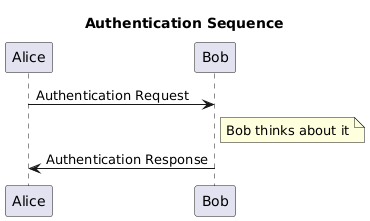
\includegraphics[width=.9\linewidth]{img/dia-001-alice-bob.png}
\end{center}


\begin{minted}[]{sh}

##
#
#

UP=1; apt update && apt upgrade; apy autoremove -y

date 


\end{minted}


\noindent\rule{\textwidth}{0.5pt}

\section{REFERENCES}
\label{sec:orgdf173c4}
\subsection{Notes}
\label{sec:orgbb4c5e4}
\begin{itemize}
\item \href{../../notes/nat/20241009T171120--30multi\_\_<meta>.org}{30multi}
\end{itemize}
\subsection{Python Standard Library}
\label{sec:orga2b5c6e}
\begin{itemize}
\item \href{https://docs.python.org/3/library/multiprocessing.html}{multiprocessing — Process-based parallelism}
\end{itemize}


\section{Refs}
\label{sec:orgc371288}
\subsection{org-refs}
\label{sec:orgd89b8e2}
print\textsubscript{bibliography}:

\subsection{bib-refs}
\label{sec:orgfb7f8e7}
\nocite{*}
\bibliographystyle{IEEEtran}
\bibliography{\xref}
\end{document}
